\documentclass[12pt, oneside]{article}

\usepackage[letterpaper, scale=0.8, centering]{geometry}
\usepackage{fancyhdr}
\setlength{\parindent}{0em}
\setlength{\parskip}{1em}

\pagestyle{fancy}
\fancyhf{}
\renewcommand{\headrulewidth}{0pt}
\rfoot{{\footnotesize Copyright Mia Minnes, 2022, Version \today~(\thepage)}}

\author{CSE105Sp22}

\newcommand{\instructions}{{\bf For all HW assignments:}

Weekly homework may be done individually or in groups of up to 3 students. 
You may switch HW partners for different HW assignments. 
The lowest HW score will not be included in your overall HW average. 
Please ensure your name(s) and PID(s) are clearly visible on the first page of your homework submission 
and then upload the PDF to Gradescope. If working in a group, submit only one submission per group: 
one partner uploads the submission through their Gradescope account and then adds the other group member(s) 
to the Gradescope submission by selecting their name(s) in the ``Add Group Members" dialog box. 
You will need to re-add your group member(s) every time you resubmit a new version of your assignment.
 Each homework question will be graded either for correctness (including clear and precise explanations and 
 justifications of all answers) or fair effort completeness. You may only collaborate on HW with CSE 105 students 
 in your group; if your group has questions about a HW problem, you may ask in drop-in help hours or post a private 
 post (visible only to the Instructors) on Piazza.

All submitted homework for this class must be typed. 
You can use a word processing editor if you like (Microsoft Word, Open Office, Notepad, Vim, Google Docs, etc.) 
but you might find it useful to take this opportunity to learn LaTeX. 
LaTeX is a markup language used widely in computer science and mathematics. 
The homework assignments are typed using LaTeX and you can use the source files 
as templates for typesetting your solutions.
To generate state diagrams of machines, we recommend using Flap.js
or JFLAP. Photographs of clearly hand-drawn diagrams may also be used. We recommend that you
submit early drafts to Gradescope so that in case of any technical difficulties, at least some of your
work is present. You may update your submission as many times as you'd like up to the deadline.


{\bf Integrity reminders}
\begin{itemize}
\item Problems should be solved together, not divided up between the partners. The homework is
designed to give you practice with the main concepts and techniques of the course, 
while getting to know and learn from your classmates.
\item You may not collaborate on homework with anyone other than your group members.
You may ask questions about the homework in office hours (of the instructor, TAs, and/or tutors) and 
on Piazza (as private notes viewable only to the Instructors).  
You \emph{cannot} use any online resources about the course content other than the class material 
from this quarter -- this is primarily to ensure that we all use consistent notation and
definitions we will use this quarter and also to protect the learning experience you will have when
the `aha' moments of solving the problem authentically happen.
\item Do not share written solutions or partial solutions for homework with 
other students in the class who are not in your group. Doing so would dilute their learning 
experience and detract from their success in the class.
\end{itemize}

}
\usepackage{amssymb,amsmath,pifont,amsfonts,comment,enumerate,enumitem}
\usepackage{currfile,xstring,hyperref,tabularx,graphicx,wasysym}
\usepackage[labelformat=empty]{caption}
\usepackage[dvipsnames,table]{xcolor}
\usepackage{multicol,multirow,array,listings,tabularx,lastpage,textcomp,booktabs}

\lstnewenvironment{algorithm}[1][] {   
    \lstset{ mathescape=true,
        frame=tB,
        numbers=left, 
        numberstyle=\tiny,
        basicstyle=\rmfamily\scriptsize, 
        keywordstyle=\color{black}\bfseries,
        keywords={,procedure, div, for, to, input, output, return, datatype, function, in, if, else, foreach, while, begin, end, }
        numbers=left,
        xleftmargin=.04\textwidth,
        #1
    }
}
{}
\lstnewenvironment{java}[1][]
{   
    \lstset{
        language=java,
        mathescape=true,
        frame=tB,
        numbers=left, 
        numberstyle=\tiny,
        basicstyle=\ttfamily\scriptsize, 
        keywordstyle=\color{black}\bfseries,
        keywords={, int, double, for, return, if, else, while, }
        numbers=left,
        xleftmargin=.04\textwidth,
        #1
    }
}
{}

\newcommand\abs[1]{\lvert~#1~\rvert}
\newcommand{\st}{\mid}

\newcommand{\A}[0]{\texttt{A}}
\newcommand{\C}[0]{\texttt{C}}
\newcommand{\G}[0]{\texttt{G}}
\newcommand{\U}[0]{\texttt{U}}

\newcommand{\cmark}{\ding{51}}
\newcommand{\xmark}{\ding{55}}
 
 
\title{HW5: Recognizability, Decidability, Undecidability, and Reductions}
\date{Due: 5/26/22 at 5pm (no penalty late submission until 8am next morning), via Gradescope}

\begin{document}
\maketitle
\thispagestyle{fancy}

{\bf In this assignment,}

You will practice designing and working with Turing machines and their variants. 
You will use general constructions and specific machines to explore the classes of recognizable, 
decidable, and undecidable languages.
You will use computable functions to relate the difficult levels of languages via mapping reduction.

{\bf Resources}: To review the topics you are working with 
for this assignment, see the class material from Weeks 6, 7, 8.
We will post frequently asked questions and our answers to them in a 
pinned Piazza post.

{\bf Reading and extra practice problems}: Chapter 4 exercises 4.1, 4.3, 4.4., 4.5. 
Chapter 4 Problems 4.29, 4.30, 4.32.  Chapter 5 exercises 5.4, 5.5, 
5.6, 5.7. Chapter 5 problems 5.10, 5.11, 5.16, 5.18.

{\bf Key Concepts}: Formal definitions of Turing machines, computations of Turing machines,
halting computations, implementation-level descriptions of Turing machines, high-level descriptions
of Turing machines, recognizable languages, decidable languages, variants of Turing machines,
enumerators, nondeterministic Turing machines, Church-Turing thesis,
 computational problems, diagonalization, undecidability, unrecognizability, 
computable function, mapping reduction.

\instructions

You will submit this assignment via Gradescope
(\href{https://www.gradescope.com}{https://www.gradescope.com}) 
in the assignment called ``HW5CSE105Sp22''.

\newpage
{\bf Assigned questions}
\begin{enumerate}
    \item ({\it Graded for correctness}\footnote{This means your solution will be
    evaluated not only on the correctness of your answers, but on your ability to 
    present your ideas clearly and logically. You should explain how you arrived at 
    your conclusions, using  mathematically sound reasoning. Whether you use formal proof techniques or 
    write a more informal argument for why 
    something is true, your answers should always be well-supported. Your goal 
    should be to convince the reader that 
    your results and methods are sound.}) 
    \begin{enumerate}
        \item Give an example of a decidable language $L_1$ whose complement is also decidable.
        A complete solution will include either (1) a precise definition of the example language $L_1$ and 
        an explanation of why it is decidable and why its complement is decidable, or 
        (2) a sufficiently general and correct argument for why there is no way to choose 
        an example language to satisfy this requirement. All justifications and arguments should
        connect to the relevant definitions and the specific concepts being discussed.
        \item Give an example of a decidable language $L_2$ and a Turing machine $M_2$ such that
        $L(M_2) = L_2$ but $M_2$ does not decide $L_2$.  A complete solution will include either (1) precise
        definitions of $L_2$ and $M_2$ and justifications for why $L(M_2) = L_2$ and why $M_2$
        does not decide $L_2$, or (2) a sufficiently general and correct argument for why there is no way to choose 
        such a language and machine. For any machines you discuss, you can choose whether to use high-level descriptions,
        implementation level descriptions, or formal definitions. All justifications and arguments should
        connect to the relevant definitions and the specific concepts being discussed.
    \end{enumerate}
    \item ({\it Graded for fair effort completeness}\footnote{This means 
    you will get full credit so long as your submission demonstrates honest 
    effort to answer the question. You will not be penalized for incorrect answers. 
    To demonstrate your honest effort in answering the question, we ask that you 
    include your attempt to answer *each* part of the question. If you get stuck 
    with your attempt, you can still demonstrate your effort by explaining where 
    you got stuck and what you did to try to get unstuck.})

    Recall that a set $X$ is said to be {\bf closed} under an operation $OP$ if, for any elements in $X$, applying 
    $OP$ to them gives an element in $X$.  For example, the set of integers is closed under multiplication
    because if we take any two integers, their product is also an integer.
    
    Suppose $M_1$  and $M_2$ are Turing machines.  Consider the following high-level  
    descriptions of machines that give general constructions based on  $M_1$  and $M_2$.
    
    \begin{enumerate}
    \item Consider the  following construction of a nondeterministic  Turing  machine:
    \begin{quote}
    ``On  input $w$
    \begin{itemize}
    \item[1.] Nondeterministically  split $w$ into two pieces, i.e. choose  $x,y$  such that  $w =  xy$.
    \item[2.] Simulate running $M_1$ on  $x$.
    \item[3.] Simulate running $M_2$ on  $y$.
    \item[4.] If both simulations in steps 2 and 3 accept, accept."
    \end{itemize}
    \end{quote}
    
    Can  this construction  be  used  to prove that the class  of  Turing-recognizable languages is closed under 
    concatenation? Briefly  justify your  answer.
    
    \item Consider the  following construction of an enumerator: 
    \begin{quote}
    ``Without any input
    \begin{itemize}
    \item[1.] Build an enumerator $E_1$ that is equivalent to  $M_1$.
    \item[2.] Build an enumerator $E_2$ that is equivalent to  $M_2$.
    \item[3.] Start $E_1$ running and start $E_2$ running.
    \item[4.] Initialize a list of all strings that have been printed by $E_1$. Declare the variable $n_1$ to be the length of  this  list 
    (initially $n_1 = 0$).
    \item[5.] Initialize a list of all strings that have been printed 
    by $E_2$ so far.
    Declare the variable $n_2$ to be the length of  this  list (initially $n_2 = 0$).
    \item[6.] Every time a new string $x$ is printed by $E_1$: 
    \item[7.] \qquad Add this string to the list of strings printed by $E_1$ so far.
    \item[8.] \qquad Increment $n_1$ so it stores the current length of the list.
    \item[9.] \qquad For $j =  1 \ldots n_2$, 
    \item[10.] \qquad \qquad Let $w_j$ be the $j$th string in the list of strings printed  by  $E_2$
    \item[11.] \qquad \qquad Print $xw_j$.
    \item[12.] Every time a new string $y$ is printed by $E_2$: 
    \item[13.] \qquad Add this string to the list of strings printed by $E_2$ so far.
    \item[14.] \qquad Increment $n_2$ so it stores the current length of the list.
    \item[15.] \qquad For $i =  1 \ldots n_1$, 
    \item[16.] \qquad \qquad Let $u_i$ be the $i$th string in the list of strings printed  by  $E_1$
    \item[17.] \qquad \qquad Print $u_i y$."
    \end{itemize}
    \end{quote}
    
    Can this construction  be  used  to prove that the class  of  Turing-recognizable languages is closed under 
    concatenation? Briefly justify your  answer.
    
    \item Consider the following construction of a Turing machine:
    \begin{quote}
    ``On input $w$
    \begin{itemize}
    \item[1.] Let  $n = |w|$.
    \item[2.] Create a two dimensional array of strings  $s_{m,j}$ where $0 \leq m \leq n$ and  $0 \leq j \leq  1$.
    \item[3.] For each  $0 \leq m  \leq n$, initialize $s_{m,0}$ to be the prefix of  $w$ of length $m$ and $s_{m,1}$ to be
    the suffix  of $w$ of length  $n-m$.  In other words, $w= s_{m,0} s_{m,1}$  and $|s_{m,0}| = m$, $|s_{m,1}| =  n-m$.
    \item[4.] For $i = 1, 2, \ldots$
    \item[5.] \qquad For $k = 0, \ldots, i$
    \item[6.] \qquad \qquad  Run $M_1$  on $s_{\min{(k,n)},0}$ for (at most) $i$ steps.
    \item[7.] \qquad \qquad  Run $M_2$  on $s_{\min{(k,n)},1}$ for (at most) $i$ steps.
    \item[8.] \qquad \qquad If  both simulations  in steps 6 and 7 accept,  accept."
    \end{itemize}
    \end{quote}
    
    Can  this construction  be  used  to prove that the class  of  Turing-recognizable languages is closed under 
    concatenation? Briefly  justify your  answer.
    \end{enumerate}

    \item ({\it Graded for fair effort completeness}) 
    Recall that 
    \[
        A_{TM} =  \{ \langle M,  w \rangle \mid \text{$M$ is a  Turing machine, 
    $w$ is a string, and $w \in L(M)$} \}
    \]
     and 
    \[
         HALT_{TM} = \{ \langle M, w \rangle \mid \text{$M$ is a Turing machine,
    $w$ is a string, and $M$ halts on $w$}\}
    \]

    Consider the Turing machines below, with input alphabet $\Sigma = \{0,1\}$, tape alphabet 
    $\{0, 1, \textvisiblespace\}$, and state diagrams (with the usual conventions):
    \begin{center}
    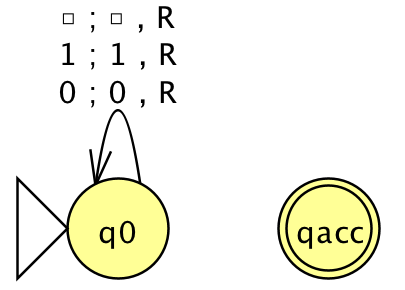
\includegraphics[width=1in]{Lect22TM1.png}\qquad\hfill \qquad
    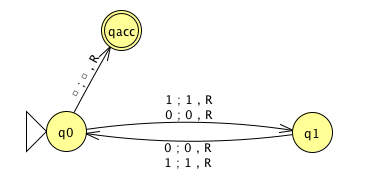
\includegraphics[width=2in]{Lect22TM2.png}
    \end{center}
    \begin{enumerate}
    \item Give an example string that is in both $A_{TM}$ and $HALT_{TM}$ and that is related to one of the 
    two Turing machines whose state diagrams are given above, or explain why there is no such string.
    \item  Give an example string that is in $A_{TM}$ and is not in $HALT_{TM}$ and that is related to one of the 
    two Turing machines whose state diagrams are given above, or explain why there is no such string.
    \item Give an example string that is not in $A_{TM}$ and is in $HALT_{TM}$ and that is related to one of the 
    two Turing machines whose state diagrams are given above, or explain why there is no such string.
    \end{enumerate}
    
    \item ({\it Graded for correctness}) Fix  $\Sigma = \{0,1\}$  for this question. 
    For each part below, you can choose sets from the  following list:  
    \[
    \emptyset, A_{TM}, \overline{A_{TM}}, HALT_{TM}, \overline{HALT_{TM}}, E_{TM}, \overline{E_{TM}}, 
    EQ_{TM}, \overline{EQ_{TM}}, \Sigma^*
    \]
    You may use each set from the list {\bf at most once} in the examples below.  In  particular, you can't choose
    $A =  B = C =  D = X = Y =  \Sigma^*$.

    
    \begin{enumerate}
    \item Find sets $A, B$ for which  the computable function
    \begin{align*}
    F &= \text{``On input $x$} \\
    &\text{1. Output $\langle 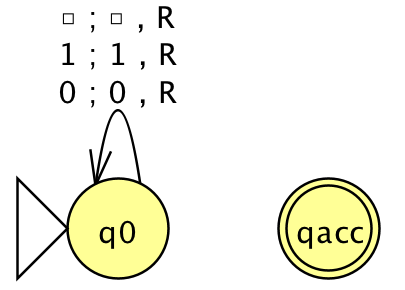
\includegraphics[width=0.5in]{Lect22TM1.png} , 00\rangle$."}
    \end{align*}
    
    witnesses the mapping reduction $A  \leq_m B$.
    Justify your  answer by  proving that, for all  strings  $x$, $x \in A $ iff  $F(x) \in B$.
    If no such sets exist, justify why not.
    
    \vfill
    
    \item Find sets $C, D$ for which  the computable function
    \begin{align*}
    G &= \text{``On input $x$} \\
    &\text{1. Check if $x = \langle M, w \rangle$ for $M$ a Turing machine and $w$ a string. If so, go to  step 3.}\\
    &\text{2. If not, output  $\langle 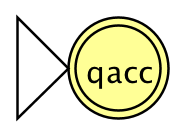
\includegraphics[width=0.5in]{hw5tm1.png},   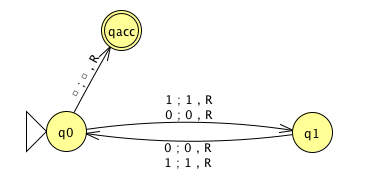
\includegraphics[width=1in]{Lect22TM2.png} \rangle$.}\\
    &\text{3. Construct the Turing machine $M'_x = $ ``On input $y$,} \\
    &\text{\qquad 1. If $y$ has a positive and odd length, reject.}\\
    &\text{\qquad 2. Else, if $y$ has a positive and even length, accept.}\\
    &\text{\qquad 3. Otherwise, run $M$ on $w$ and, if the computation halts, accept $y$."}\\
    &\text{4. Output  $\langle M'_x , 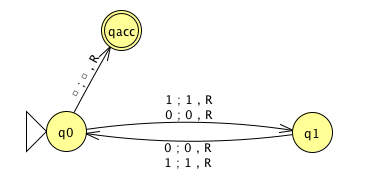
\includegraphics[width=1in]{Lect22TM2.png}\rangle$."}
    \end{align*}
    
    \vspace{-10pt}
    
    witnesses the mapping reduction $C  \leq_m D$.
    Justify your  answer by  proving that, for all  strings $x$, $x \in C $ iff  $G(x) \in D$.
    If no such sets exist, justify why not.

    
    \vfill
    
    \item Find sets $X, Y$ for which  the computable function
    \begin{align*}
    H &= \text{``On input $x$} \\
    &\text{1. Check if $x = \langle M, w \rangle$ for $M$ a Turing machine and $w$ a string. If so, go to  step 3.}\\
    &\text{2. If not, output  $\langle 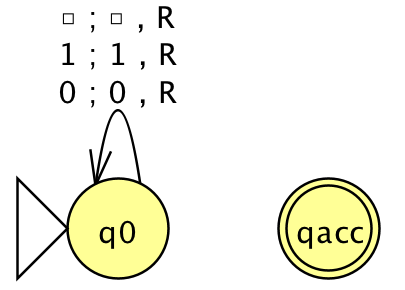
\includegraphics[width=1in]{hw5tm2.png}\rangle$.}\\
    &\text{3. Construct the Turing machine $M'_x = $ ``On input $y$,} \\
    &\text{\qquad 1. If $y \neq w$, reject.}\\
    &\text{\qquad 2. Otherwise, run $M$ on $w$.}\\
    &\text{\qquad 3. If $M$  accepts,  accept.  If  $M$ rejects, reject."} \\
    &\text{4. Output  $\langle M'_x \rangle$."}
    \end{align*}
    
    \vspace{-10pt}
    
    witnesses a mapping reduction $X \leq_m Y$. 
    Justify your  answer by  proving that, for all  strings $x$, $x \in X $ iff  $H(x) \in Y$.
    If no such sets exist, justify why not.
    
    \end{enumerate}
\end{enumerate}
\end{document}